\cotefile{148}

% 148_scan048
\scanpage{48}
\mspage{4)}
On a un foncteur
\diagram{\begin{tikzcd}[ampersand replacement=\&]
(*)\quad\Gamma:\quad S_*\mathcal TD^\pm_{\mathrm{top}}\arrow[r]\&
\deleted{\unsure{\mathrm{F}}\mathrm{MD}}(\mathrm{Gra\,bipond})
\end{tikzcd}}
qui associe à un objet \inserted{$(X,\widetilde\Sigma,R)$} de
$S_*\mathcal TD^\pm_{\mathrm{top}}$ le graphe \inserted{MD}
$(S,\vec A,\sigma,\deleted{\unsure{g}}\inserted{\unsure{o|\sigma}},\deleted{\unsure{)}}\gamma,\rho)$ suivant :
\[
S=\pi_0(X\deleted{\unsure{)|,}}\setminus\widetilde\Sigma)\xleftarrow{\sim}\pi_0(\text{Déc}(X,\widetilde\Sigma))
\]
$\vec A=$ ens des couples $(C,\deleted{\unsure{\xi}}\omega)$, où
$C$ \deleted{\unsure{$\in A$|est un}}\inserted{$\in\pi_0(\widetilde\Sigma)$}, et où
$\omega\in\mathrm{Or}(C)\inserted{\simeq\mathrm{rive}_X(C)}$,
soumis à la condition que si $C\in\pi_0(\partial X)$, \unsure{alors|donc} $\omega$
soit l'orientation induite i.e. la rive qui se trouve dans $X$

$\sigma=$ échange des rives (quand on a le droit d'échanger,
sinon, i.e. si $C\in\pi_0(\partial X)$, on pose $\sigma(a)=a$)

$\deleted{\unsure{O}}\inserted{o}$ : associe à $(C,\text{rive de }C)$
l'unique ``face'' $\in\pi_0(X\setminus\widetilde\Sigma)$ qui
\deleted{$\unsure{R\subset\widetilde R}$} contient cette rive
\diagram{\begin{tikzcd}[ampersand replacement=\&]
\gamma:\quad S\arrow[r]\arrow[d,equal]\&\mathbb N\\
\pi_0(X\setminus\widetilde\Sigma)\&
\end{tikzcd}}
application \uline{genre} des composants $X_i$.
\diagram{\begin{tikzcd}[ampersand replacement=\&]
\deleted{\unsure{\rho}}\inserted{r}:\quad A=\pi_0(\widetilde\Sigma)\arrow[r]\&\mathbb N\&
:\quad C\arrow[r,mapsto]\&\mathrm{Card}(R\cap C).
\end{tikzcd}}

Le foncteur $(*)$ \deleted{est \uline{ess. surjectif} et}
\inserted{induit un \uline{iso} sur les} $\pi_0$ et une surjectif
sur les $\pi_1$ (c'est un \uline{0-isomorphisme} \deleted{\unsure{)|?}},
en langage homotopique).

\deleted{\unsure{Prop.|La preuve}} :

\uline{Remarques}. Dans $S_*\mathcal TD^\pm_{\mathrm{top}}$ il y a une
opération évidente de \uline{somme} \inserted{\uline{directe}},
dans $\deleted{\mathrm{FMD}}\inserted{\mathrm{Gra\,bipond}}$ aussi,
et $(*)$ y commute.
\mspage{47}

% 148_scan049
\scanpage{49}
\mspage{5)}
Cette opération de \unsure{somme|sommes} est la plus triviale parmi les opérations qu'il
nous faudra expliciter et transcrire (combinatoirement) dans la suite.
Notons de suite, pour $(X,\widetilde\Sigma,R)$, donné
\[
X\deleted{\unsure{est}}\text{ connexe}\Longleftrightarrow
\Gamma\mathrm{MD}(X,\widetilde\Sigma,R)\text{ connexe}
\]
plus précisément
\[
\pi_0(X)\simeq\pi_0(\Gamma\mathrm{MD}(X,\widetilde\Sigma,R))
\]
\margin{donner la formule pour le genre d'un
$\alpha\in\pi_0(X)\simeq\pi_0(\Gamma)$ en termes de la pondération ---
plus généralement le \uline{genre total} est
\figure{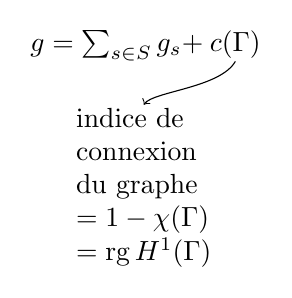
\begin{tikzpicture}[baseline,scale=.85]
\node[anchor=base east,inner sep=1pt] at (0,0) {$g=\sum_{s\in S}g_s+$};
\node[anchor=base west,inner sep=1pt] (c) at (0,0) {$c(\Gamma)$};
\node[anchor=north west,align=left,inner sep=1pt] (note) at (-2,-.8)
{indice de\\connexion\\du graphe\\
$\deleted{\unsure{=1-\chi(\Gamma)}}$\\
$\inserted{=\mathrm{rg}\,H^1(\Gamma)}$};
\draw[->] (c.south) .. controls (.2,-.55) and (-.8,-.6) .. (note.north);
\end{tikzpicture}}}

\uline{Cas particuliers.}

a) Cas de $S_*\mathcal T^\pm_{\mathrm{top}}\
\deleted{\unsure{S_*\mathcal T_{\mathrm{top}}}}$
--- i.e. $\Sigma=\phi$, $\widetilde\Sigma=\partial X$.

Cela correspond au cas des graphes MD \deleted{que} où
\inserted{toutes les arêtes sont libres, i.e.}
tous les sommets sont isolés (sauf arêtes libres)
\deleted{Il} \inserted{Ce graphe} est donc déterminé par
\diagram{\begin{tikzcd}[ampersand replacement=\&,column sep=large]
A\ (\simeq\vec A=\vec A^\sigma)\arrow[r,"r"]\arrow[d]\&\mathbb N\\
S\arrow[r,"\gamma"]\&\mathbb N
\end{tikzcd}}

Le cas de $\mathcal T^\pm_{\mathrm{top}}$ correspond : choisir $\rho=0$,
donc la situation est donnée par
\diagram{\begin{tikzcd}[ampersand replacement=\&]
A=A_0\arrow[d]\&\\
S\arrow[r,"\gamma"]\&\mathbb N.
\end{tikzcd}}

\margin{\figure{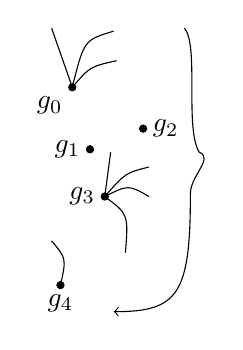
\begin{tikzpicture}[scale=.75]
\fill(0,0)circle(2pt);\node[below left]at(0,0){$g_0$};
\draw(0,0)--(-.35,1) (0,0)..controls(.2,.8)..(.7,.95)
(0,0)..controls(.3,.35)..(.75,.45);
\fill(.3,-1.05)circle(2pt);\node[left]at(.3,-1.05){$g_1$};
\fill(1.2,-.7)circle(2pt);\node[right]at(1.2,-.7){$g_2$};
\fill(.55,-1.85)circle(2pt);\node[left]at(.55,-1.85){$g_3$};
\draw(.55,-1.85)--(.65,-1.1)
(.55,-1.85)..controls(.9,-1.45)..(1.3,-1.35)
(.55,-1.85)..controls(.95,-1.65)..(1.3,-1.85)
(.55,-1.85)..controls(.95,-2.15)..(.9,-2.8);
\fill(-.2,-3.35)circle(2pt);\node[below]at(-.2,-3.35){$g_4$};
\draw(-.2,-3.35)..controls(-.1,-2.9)..(-.35,-2.6);
\draw[->](1.9,1)..controls(2.15,.7)and(1.9,-.7)..(2.15,-1.1)
..controls(2.4,-1.2)and(2,-1.5)..(2,-1.8)
..controls(2,-3.5)and(1.8,-3.8)..(.7,-3.8);
\end{tikzpicture}}}

\inserted{Le cas d'une} \uline{structure} connexe
$(\mathrm{card.}\,S=1\inserted{\text{ i.e. }S=\{s\}})$
\deleted{type $(g,\nu)$ d'une}
est \deleted{\unsure{Déterminé}}
\unsure{\deleted{\inserted{caractérisé}}|\inserted{caractérisé}}
par \deleted{\unsure{le genre}} la donnée des deux entiers $(g,\nu)$
$(g=\text{genre},\ \nu=\text{nb de trous})$
\[
g=\gamma(s),\qquad \nu=\mathrm{card}\,A
\]
\mspage{48}

% 148_scan050
\scanpage{50}
\mspage{6}
\uline{Remarque} En fait, on a un foncteur plus précis, vers une catégorie de graphes munis d'une structure où la partie $\rho$ de la pondération est \deleted{\unsure{complétée}} \inserted{remplacée} par une structure plus précise, à savoir \deleted{une \unsure{application}} \inserted{une \deleted{\unsure{famille}}} famille
\deleted{\diagram{\begin{tikzcd}[ampersand replacement=\&,row sep=small,column sep=small]
A\,(\widetilde R,\alpha,\unsure{p|\rho}:R\arrow[r]\&\vec A\,)\arrow[d,equal]\\
\&\vec A/\sigma
\end{tikzcd}}}
\[
 (R_a)_{a\in A}
\]
\margin{$\omega(a)\mathrel{\mathop=^{\rm def}}\{\vec a\in\vec A/\vec a\text{ au dessus de }a\}$}
d'ensembles, et pour $\forall a\in A$, si $\omega(a)$ désigne l'\unsure{ens|un} des
\deleted{\unsure{donné d'une permutation de}}
``orientations'' de $a$ ($\operatorname{card}\omega(a)\in\{1,2\}$), une application
\deleted{$R$, et $\unsure{p|\rho}$ une application $R\longrightarrow A$ \unsure{conj. à}}
\[
 \omega\longmapsto u_\omega:\quad \omega(a)\longrightarrow\operatorname{Circ}(R_a)
\]
ens des permutations circulaires sur $R_a$
\deleted{et \unsure{d'autre} \unsure{une} \unsure{\illegible{1} une application injective|application injective}}
\[
 \deleted{R/\alpha\lhook\joinrel\longrightarrow\vec A}
\]
avec la condition que si $\omega,\omega'\in\omega(a)$, $\omega\ne\omega'$, alors
\[
 \deleted{u_\omega u_{\omega'}=\operatorname{id}_{\unsure{R_a|R}}}
 \qquad u_{\omega'}=u_\omega^{-1}
\]

On peut aussi considérer que la donnée des suppléments revient à la donnée de
\[
 \begin{array}{r@{}c@{}l}
 &r&:A\longrightarrow\mathbb N\\[-.3ex]
 &\Vert&\\[-.3ex]
 a\longmapsto&\operatorname{Card}&\unsure{p|\rho}^{-1}(a)
 \end{array}
\]
(la ``pondération-arêtes''), et la donnée d'une famille de torseurs
\[
 (R_a)_{a\in A},\quad \deleted{\unsure{\omega(a)}}
\]
$R_a$ un torseur sous $\mathbb Z/r(a)\mathbb Z\mathbin{\wedge}^{\omega(a)}_{\{\pm1\}}$
On associe à $(X,\widetilde\Sigma,R)$ une telle structure supplémentaire :
\[
 R_a=R\cap\widetilde\Sigma_a
\]
($\widetilde\Sigma_a$ la comp. connexe de $\widetilde\Sigma$ \deleted{\unsure{marquée}} \inserted{qui correspond à} $a\in A\simeq\pi_0(\widetilde\Sigma)$),
\deleted{$\unsure{R=R(\Sigma C)|R=\pi_0(\widetilde\Sigma)}$,}
\deleted{\diagram{\begin{tikzcd}[ampersand replacement=\&,row sep=small,column sep=large]
R\arrow[r]\arrow[d,equal]\&S\arrow[d,equal]\\
\unsure{\Gamma}\arrow[r]\&\pi_0(\widetilde\Sigma)
\end{tikzcd}}}
\deleted{\unsure{la donnée de} $\widetilde\Sigma$}
$\omega\longmapsto u_\omega$ défini de façon évidente.
\deleted{et $\unsure{p|\rho}$ déduit de l'ordre circulaire \unsure{dans|sur} les $R_a$}

\uline{NB} Même si $r(\omega)=1$ ou $r(\omega)=2$, le fait de disposer
\mspage{49}

% 148_scan051
\scanpage{51}
\mspage{\deleted{\unsure{6}}7}
d'une structure déjà orientée si $a$ est une arête libre
(correspondant à un $C\in\pi_0(\partial X)$), ou qu'on dispose
\unsure{\inserted{de}|de} l'une des deux orientations $\omega(a)$ ---
dans le cas où $a$ est une arête ordinaire, indique que l'on tient en mains,
pour chaque $a\in A$, un polygone combinatoire $P_a$, dont l'ens des sommets
est $R_a$, et l'ens des arêtes peut se décrire \deleted{\unsure{aussi}}
de façon canonique en termes de $R_a,\omega_a$ et
$\omega_a\longrightarrow\operatorname{Circ}(R_a)$.
Il peut être plus commode de la donner d'emblée dans la structure,
où la famille des $(R_a)$ serait remplacée par un
\deleted{qui serait \unsure{dans un contour|les uns un contour}}
\uline{contour combinatoire}, i.e. un ensemble de repères
$\vec{\underline R}$ (plutôt ``repères de rigidification''), avec une opération de
\[
 \mathbb D_\infty=\{\sigma_0,\sigma_1\mid\sigma_0^2=\sigma_1^2=1\}
\]
dessus, et une application
\[
 \vec{\underline R}\longrightarrow\vec A
\]
compatible avec l'hom.
\[
 \mathbb D_\infty\xrightarrow{\varepsilon}\{\pm1\}
\]
sur les groupes d'opérateurs, mais de plus un sous ens
\[
 \vec{\underline R}_l^+\subset\vec{\underline R}\mid\vec A_l
\]
\margin{$(\vec A_l=\text{arêtes libres, correspondant aux cercles de recollements, i.e. les }\in\pi_0(\unsure{\partial}X))$}
définissant une orientation des contours correspondant.
\mspage{50}

% 148_scan052
\scanpage{52}
\mspage{8}
On a ainsi la notion de \uline{graphe pondéré} \deleted{\unsure{enrichi}} \inserted{\uline{à repères}} $\Gamma$

\diagram{\begin{tikzcd}[ampersand replacement=\&,column sep=large,row sep=large]
\vec R_l^+\ \deleted{\unsure{\mathbb D_\infty|D_\infty}}\subset\underset{\sigma_0,\sigma_1}{\vec R}
 \arrow[r]\&\vec A\arrow[d,"o"']\arrow[loop right,"\sigma"]\\
\&S\arrow[r,"\gamma"]\&\mathbb N
\end{tikzcd}}

Groupoïde (\uline{Gr.pndrep})

foncteur
\[
 S_*\mathcal TD_{\mathrm{top}}^\pm\longrightarrow(\mathrm{Grpondrep})
\]
qui sera importante sans doute dans l'explicitation de l'opération de ``recollement''.
Il est clair en tous cas que toute description-traduction algébrico-combinatoire de
$S\mathcal TD_{\mathrm{top}}^\pm$ devra permettre, pour chaque objet de
\deleted{la catégorie} \inserted{gr.poïde-}paradigme, de réconstituer (à isom. uniques près) le \uline{graphe pondéré à repères} correspondant.
\inserted{--- plus précisément, il faut réconstituer le foncteur canonique
$S_*\mathcal TD_{\mathrm{top}}^\pm\longrightarrow(\mathrm{Gr.pond.rep.})$
(et non seulement le foncteur à valeurs dans $(\mathrm{Grbipond})$)}

\uline{Opérations essentielles}

A) Opérations ``d'oubli'' ou de ``\uline{gommage}''.

\textcircled{1} \uline{Gommage des repères} À un objet $(X,\Sigma,R)$, muni en plus d'une partie $R'\subset R$, il associe $(X,\Sigma,R\setminus R')$ (gommage de $R'$).
\mspage{51}

% 148_scan053
\scanpage{53}
\mspage{9}
\uline{NB} Ayant (via un groupoïde équivalent à description purement combinatoire) ``réconstruit''
\deleted{\unsure{ou|du}} \deleted{\unsure{plutôt|purement}} réalisé le groupoïde
$S\mathcal TD_{\mathrm{top}}^\pm$, et le foncteur
\[
 S\mathcal TD_{\mathrm{top}}^\pm\longrightarrow(\mathrm{Gr.\ pond.\ rep})
\]
\deleted{\unsure{alors}} on aura \deleted{\unsure{par}} donc aussi \deleted{\unsure{une description}} \inserted{l'équivalent de}
\deleted{de} la donnée d'un $(X,\Sigma,R)$, muni \uline{en plus} d'une partie $R'\subset R$ --- \deleted{d'où} i.e. avec la construction d'un groupoïde \unsure{équivalent|au-dessus}
\diagram{\begin{tikzcd}[ampersand replacement=\&,row sep=large]
S_*\mathcal TD_{\mathrm{top}}^\pm\,
 \begin{gathered}(\text{à sous ens. marqué }R')\\
 \text{de sommets-}\\\text{repères}\end{gathered}\arrow[d]\\
S_*\mathcal TD_{\mathrm{top}}^\pm
\end{tikzcd}}
et \deleted{\unsure{d'où}} il nous faudra donc \inserted{décrire} un foncteur ``gommage de $R'$''
\diagram{\begin{tikzcd}[ampersand replacement=\&,column sep=huge]
S_*\mathcal TD_{\mathrm{top}}^\pm
 \left(\underset{\text{marqué}}{\overset{\text{ens}}{\deleted{\unsure{R_0|R}}R'}}\right)
 \arrow[r,"\text{gommage de }R'"]\arrow[r,shorten >=4em]
 \&S_*\mathcal TD_{\mathrm{top}}^\pm
\end{tikzcd}}
\deleted{Cela s'exprime, sur le}
donnant lieu : un diagramme comm. de foncteurs
\diagram{\begin{tikzcd}[ampersand replacement=\&,row sep=large,column sep=large]
S_*\mathcal TD_{\mathrm{top}}^\pm(\ldots R'\ldots)
 \arrow[rr,"\text{gommage de }R'"]
 \arrow[d,"\begin{gathered}\text{oubli du }\deleted{\unsure{R'}}\text{ marquage}\\R'\end{gathered}"]
 \&\&S_*\mathcal TD_{\mathrm{top}}^\pm\arrow[ddl]\\
S_*\mathcal TD\deleted{\unsure{\#}}_{\mathrm{top}}^\pm\arrow[dr]\&\&\\
\&(\mathrm{Gra}\deleted{\unsure{\mathrm{bi}}}\mathrm{pond})
 \arrow[r]\&
 \begin{gathered}\text{graphes avec}\\\text{pondération}\\
 \text{par }\gamma,\text{ mais}\\\text{non par }r,\end{gathered}
\end{tikzcd}}
alors qu'au niveau

\margin{\uline{NB} Cette opération a l'air d'un \uline{affaiblissement} de structure --- mais cet affaiblissement, \unsure{sur|pour} une composante $C$ donnée de $\Sigma^+$, lorsqu'on ``gomme'' \uline{tous} les repères de \deleted{\unsure{ce}} $C$ --- sinon c'est au contraire plutôt dans le sens d'un renforcement de structure, --- ou plutôt, des \unsure{marquages|groupoïdes} \unsure{qui} \unsure{du nombre de|du même type} $R'_C=R'\cap C$, dans le cas catégories isotopiques \deleted{\unsure{au dessus de}} \inserted{l'opération de gommage et celles} de surmarquage (\unsure{cf.} plus bas) \unsure{correspondantes} sont inverses \unsure{l'une de l'autre|l'un de l'autre}, sont des équivalences de groupoïdes.
Il faudrait séparer les deux cas, pour distinguer ces \uline{opérations de gommage essentielles} (qui changent le groupe des autom.) et les autres.}
\mspage{52}

% 148_scan055
\scanpage{55}
\mspage{11}
3) \deleted{Gommage} \inserted{Bouchage de trous, ou ``gommage''} de cercles de recollement.

Cette opération est relative à la donnée d'une 1-sous-variété fermée de $\partial X$, i.e. d'une partie $A'_l$ de $\pi_0(\partial X)\simeq A_l$ (ens des arêtes libres du graphe).
Elle consiste à boucher les trous correspondants, au moyen des cônes sur les composantes connexes du bord de $\Sigma'_l$.
Au niveau du graphe, cela consiste à gommer les arêtes libres correspondantes, avec bien entendu aussi les repères de marquage qui se trouvent au dessus --- \deleted{mais} les pondérations des sommets restent inchangées.

\deleted{\unsure{4)}}
\uline{Gommage simultané mixte}, \deleted{\unsure{ou}} correspondant à une partie
\deleted{\inserted{$A'\amalg R'$}} \inserted{$R'\amalg\Sigma'$} \deleted{quelconque} \inserted{de $R\amalg\Sigma$} \deleted{des}
qui soit à la fois ouverte et fermée \deleted{\unsure{que}} \inserted{et telle}
\deleted{\unsure{de} $A\amalg R$}\unsure{,}
\inserted{que $R'\supset R\cap\Sigma'$},
\deleted{\unsure{un} ens. de composantes connexes de $R\amalg\Sigma$}\unsure{,}
ou ce qui revient au $=$, une partie \inserted{$R'\amalg A'$} de $R\amalg A$, telle que $R'\supset R\mid A'$.

Au niveau des graphes pondérés à repères, cette opération consiste à enlever \unsure{\deleted{les}|la} \inserted{de $\vec R$} partie corr. $\vec R'$, à contracter en un point les arêtes de $A'_{\deleted{\unsure{pq}}}$ (aussi bien libres que liées), en faisant suivre la pondération.
\mspage{54}

% 148_scan056
\scanpage{56}
\mspage{12}
\fbox{\deleted{\unsure{A)|4)}}} \inserted{(B)}
\uline{Opération} \uline{de} \deleted{\uline{affaiblissement \unsure{et|ou}} de} \inserted{\uline{sur}}\uline{marquage}

\deleted{On peut le définir \inserted{en termes de} par la donnée, d'une \inserted{\unsure{composante connexe de}} pour chaque arête du contour $R$ \unsure{$R\ne\phi$} $\widetilde\Sigma\setminus R$ Soit $\unsure{\widetilde\Sigma_*}\;A_0^+\unsure{\subset|\in}\unsure{A_0|A_*}$ l'ens}
\deleted{\unsure{des}}
Soit $A^+$ l'ens des arêtes \inserted{(libres ou liées)} ``effectivement marquées'', \inserted{du $\Gamma$ bip. telles que $r(a)>0$},
\deleted{et $B$ l'ens des},
correspondant à des $C\in\pi_0(\Sigma)$ telles que $C\cap R\ne\phi$, soit $B^+$ l'ens des comp. connexes \unsure{des|de}
\[
 \Sigma^+\setminus R\cap\Sigma^+
\]
(lesquelles sont des int. ouverts), un surmarquage est défini par la donnée d'une application
\[
 B^+\xrightarrow{r'}\mathbb N,
\]
et peut se décrire \deleted{par} \inserted{comme} l'opération qui sur chaque
\uline{arête} \inserted{\unsure{(ouverte)|\deleted{(ouverte)}} \deleted{qui}}
de $\Sigma$, correspondant à un $b\in B^+$, $r'(b)$ nouveaux sommets de \deleted{\unsure{marquage}} \inserted{rigidification}.
Cette fois-ci, \deleted{\unsure{l'opé}} il y a des choix arbitraires --- néanmoins l'opération donne un objet de $S\mathcal TD^+$, défini à isom unique près \inserted{soit $(X,\Sigma,R_1)$} --- muni bien entendu d'un ens marqué $R'\subset R_1$, tel que l'opération inverse de gommage de $R'$ redonne l'objet de départ $(X,\Sigma,R)$.

\margin{\deleted{arêtes} cercles \deleted{\unsure{marqués}} \inserted{effectivement} marqués, \inserted{corr.} \uline{arêtes} sur $\Sigma$ \unsure{que}}
\margin{(\uline{NB} elles \unsure{sont les intersections|se trouvent sur|se déduisent} des cercles eff. marqués, et sont des intervalles ouverts)}
\mspage{55}
